\documentclass[colorlinks=true,pdfstartview=FitV,linkcolor=blue,
            citecolor=red,urlcolor=magenta]{ligodoc}

\usepackage{graphicx}
\usepackage{amssymb}
\usepackage{amsmath}
\usepackage{longtable}
\usepackage{rotating}
\usepackage[usenames,dvipsnames]{color}
\usepackage{fancyhdr}
\usepackage{subfigure}
\usepackage{hyperref}
\ligodccnumber{T}{11}{XXXXX}{}{vX}% \ligodistribution{AIC, ISC}


\title{Data Mining Techniques for Classification of Environmental Noise in LIGO Detectors}

\author{Jacob Bernhardt}

\begin{document}

% A research plan of two or three pages, carefully thought out and precisely worded, should be sufficient to make all the important points. Concerning structure and content: start out with the sections indicated below and try to answer the questions provided in each part. When you have this material developed, you may be able to reorganize it so that it flows more logically while covering the same ground.

\section{Introduction}
% What is the general technical area in which you will be working? What is the problem that you are trying to solve, and how did the problem arise? Why is its solution interesting or worthwhile? What is the status of related research by your mentor or by the group that you will be joining, and what will be the contribution and significance of your effort if it is successful?
The LIGO project uses laser interferometery to measure transverse gravitational waves.
When a gravitational wave passes, it changes the relative lengths of a LIGO detector's two orthogonal resonating RF cavities, creating a signal in the DARM (differential arm) channel.
Due to amplitude scales of these astronomical waves, the current 4-km detectors have to operate at a very low signal-to-noise ratio (SNR).
The design of 4-km LIGO is thus heavilly focused on treatment of noise.

To help identify and characterize environment-based noise, a LIGO detector has a Physical Environment Monitoring (PEM) system, a diverse array of environmental sensors positioned all over the facility.
This is used for a multitude of purposes, including the data quality report (DQR) used for time segment vetoing, based on direct statistical correlation of PEM channels to DARM.
Supplementing coincidence analysis between the two detectors, DQR prevents gravitational wave-like noise transients from being falsely categorized as events.
While vetoing and determining signal quality is useful, detector livetime can be increased by adding mechanical, electrical, or software-based components that directly remove environmental noise from the gravitational wave channel.
However, noise doesn't always affect dedicated sensors the same way as it does DARM; there may be some frequency conversion.
Noise injections (e.g. speaker, seismic shaker) are sometimes performed to get a ``coupling function''\cite{pemcoupling} for each source into the detector, but even after automated calibration, the noise is not completely removed. There are many unpredictable or hard-to-model effects of real noise which can't be found by injection.
\begin{figure}
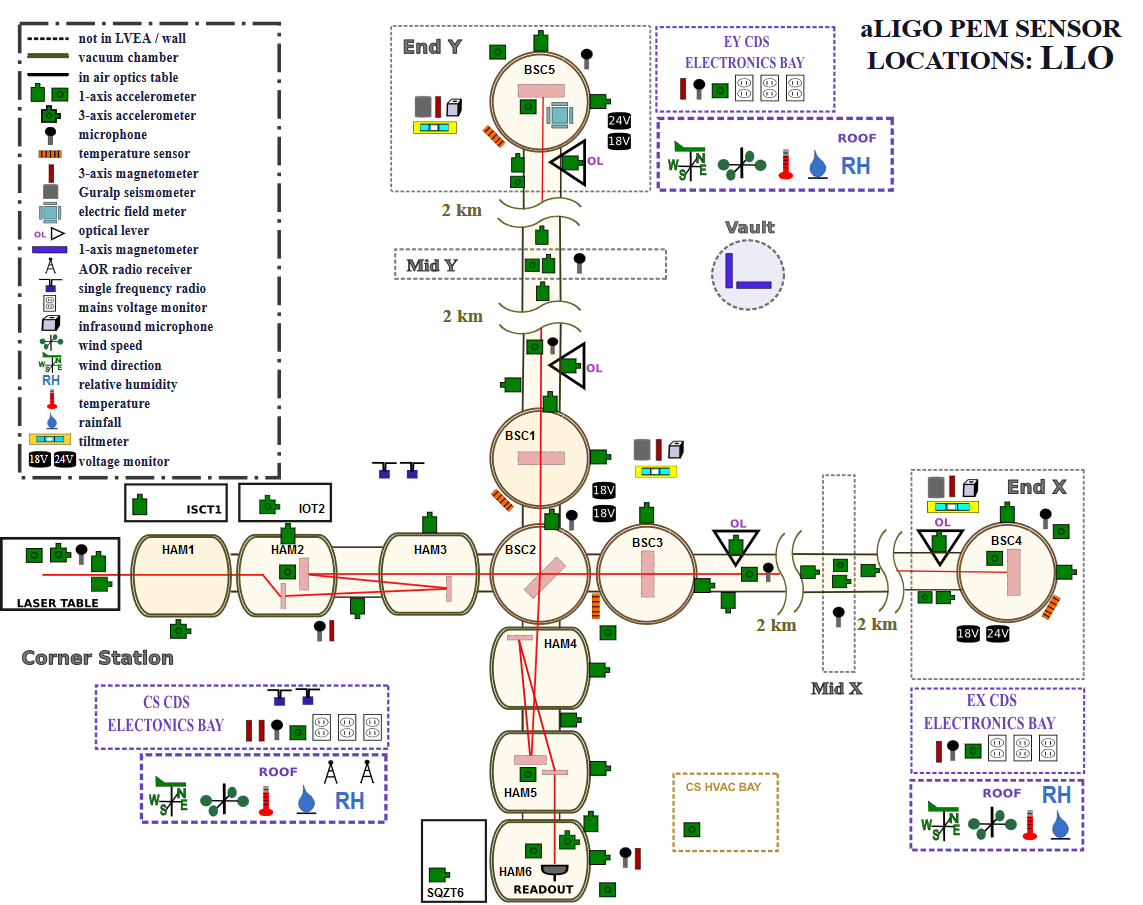
\includegraphics[width=\textwidth]{llopem.png}
\caption{Schematic PEM map at the LIGO Livingston Observatory. Shaded areas are in vacuum.}
\end{figure}

Noise sources appear in a range of different frequency bands, so separating noise sources out of a signal is a clustering problem in frequency space.
A previous LIGO SURF student has evaluated several data clustering algorithms with respect to their ability to properly sort out frequency elements of seismometer signals caused by specific earthquake events\cite{roxana}.
Both the \texttt{k-means} algorithm, which aims to make clusters with low standard deviation, and the \texttt{dB-scan} algorithm, which minimizes overall inter-point distance in clusters, were evaluated using multiple methods, including the Calinsky-Harabaz  index and direct comparison to earthquake times via time labeling of points, ultimately showing poor earthquake identification.
A long short-term memory (LSTM) recurrent neural network (RNN) seemed to work much better, but due to small input sample size, this solution may have been be plagued by over-fitting.
Thus, it is imperative that a more robust frequency clustering mechanism be designed for the PEM system.

\section{Objectives}
% What do you aim to accomplish in your project? What will you measure, and under what conditions; or, what will you calculate, model, or simulate; or what will you design, and what are the requirements; or what will you build or test? What is your starting point? What are your initial assumptions or conditions? What will be the result or product of a successful outcome for your project? What are the criteria for project completion or for success? (In other words, how will you know when you have accomplished what you set out to do?)
\begin{itemize}
\item
As a primary goal, \textbf{algorithms or clustering approaches which correctly identify labeled noise events need to be found}.
As every algorithm has inbuilt assumptions about the dataset it is applied to, the results of an algorithm performance test on labeled data will yield information about the structure of the data.
The general temporal nonstationarity of the DARM noise will need to be accounted for by varying testing time windows.
\item
The secondary goal is to \textbf{use the uncovered structure (or lack thereof) to inform a clustering approach designed to be applicable on partially labeled or unlabeled data}.
This is where the ``detector characterization tool'' that this project aims to advance will be functional---achievement of this goal means ability to reveal new and previously unknown coupling pathways between ambient noise sensors and DARM, and therefore also the ability to design new noise-filtering components to put in the detector.
\end{itemize}

\section{Approach}
% Specifically, how will you reach your objective or produce your desired final product? What are the principal steps or milestones along the path? How long will each take? What steps promise to be the most difficult, and how will you overcome the difficulties? What equipment or other resources will you need? Which of these are inherited, and which will you have to make or procure? With what other people or groups will you be collaborating? Will completion of your project depend on results from other people in related projects? (That question may be especially pertinent for team projects.)

Initially, a program will be written to take the spectral power of any PEM channel, in the form of band-limited RMS (BLRMS), likely using established methods like looping through a smoothed spectogram of the channel\cite{vajente}.

To reach the first objective, a modular \texttt{python} testing suite will be written to probe the structure of the multidimensional frequency-domain sensor data.
This will strategically implement \texttt{scikit-learn} clustering algorithms and classifiers with different optimal regimes of function or working assumptions and evaluate them using point labeling. 
This will require, additionally to researching clustering or unsupervised classification algorithms, thinking of as many variables which may affect the data structure and intelligently testing them. 
Optimizations will need to be considered so that run times are reasonable.

The program tackling the second objective will have a form dependent on the results of the first objective.
It is unlikely that a certain algorithm or technique outperforms the rest for all types of sensory data, so the final program will use the modular programming environment created for the testing suite to match techniques to the regimes that they work in.
The structure of the input data as determined by the first objective, including the dimensionality probed by the extra variables, may lend itself to additional algorithms that can be used to combine the target regimes.
To this end, extra algorithm research will be conducted with specific consideration of the solved structure.


\section{Project Schedule}
% Preparing a schedule of the principal activities and events is a good way of showing the readers that you have taken a systematic approach to planning your work.
\paragraph{Before Arrival}
\begin{itemize}
\item Research algorithms to use
\item Develop glitch-resistant BLRMS-making code
\item Continue familiarizing with \texttt{scikit-learn} by adapting old clustering code for beamtube accelerometers
\end{itemize}
\paragraph{Week 1-2}
\begin{itemize}
\item Familiarize with types of PEM data that can have labeled events
\item Complete the algorithm testing suite
\end{itemize}
\paragraph{Week 3-4}
\begin{itemize}
\item Develop ways to plug channels into the suite
\item Run suite on determined variety of channel combinations and regimes
\end{itemize}
\paragraph{Week 5-6}
\begin{itemize}
\item Examine results, decide next steps
\item Research new algorithms
\item Adapt initial codebase for application
\end{itemize}
\paragraph{Week 7-8}
\begin{itemize}
\item Try to reveal new PEM-DARM coupling mechanisms and propose/implement solutions
\end{itemize}
\paragraph{Week 9-10}
\begin{itemize}
\item Finish up final analysis and writing final report.
\end{itemize}

\begin{thebibliography}{3}
\bibitem{roxana} LIGO Document T1700198-v1
\bibitem{vajente} aLIGO LLO Logbook entry 45374 by Gabriele Vajente
\bibitem{pemcoupling} See \url{http://pemcoupling.readthedocs.io} for the code that does this.
\end{thebibliography}
% List all pertinent papers or reports that you have consulted to prepare your plan. Include remarks or suggestions from your prospective supervisor, from graduate students, or from other people with whom you have talked.

\end{document}
 
